\documentclass[12pt]{article}

% --- Pacotes Fundamentais ---
\usepackage[brazilian]{babel}
\usepackage[utf8]{inputenc}
\usepackage[T1]{fontenc}
\usepackage{amsmath, amsfonts, amssymb}
\usepackage{graphicx}
\usepackage{url}
\usepackage{geometry}
\usepackage{booktabs}
\usepackage{float}
\usepackage[table,xcdraw]{xcolor}
\usepackage{longtable}
\usepackage{fancyvrb}
\usepackage{hyperref}

% --- Configurações de Margem (ABNT) ---
\geometry{a4paper, left=3cm, top=3cm, right=2cm, bottom=2cm}

% --- Cores Customizadas ---
\definecolor{lightgray}{gray}{0.95}
\definecolor{headergray}{gray}{0.2}

% --- Macro para Histórias de Usuário ---
% Uso: \userstory{ID}{Título}{Requerente}{Ação}{Comentários}{CA}{RN}{RNF}{Prioridade}
\newcommand{\userstory}[9]{
\begin{table}[H]
\centering
\small
\begin{tabular}{|l|p{10.5cm}|}
\hline
\rowcolor{gray!20} \textbf{ID} & \textbf{#1} \\ \hline
\textbf{Título} & #2 \\ \hline
\textbf{Requerente} & #3 \\ \hline
\textbf{Ação} & #4 \\ \hline
\textbf{Comentários} & #5 \\ \hline
\textbf{Critérios de Aceitação} & #6 \\ \hline
\textbf{Regras de Negócio} & #7 \\ \hline
\textbf{RNF / Prioridade} & #8 / Prioridade: \textbf{#9} \\ \hline
\end{tabular}
\caption{Cartão de História de Usuário - #1}
\end{table}
}

\begin{document}

% ----------------------------------------------------------------------------------------
%	CAPA
% ----------------------------------------------------------------------------------------
\begin{titlepage}
    \center
    \textsc{\Large Universidade Cruzeiro do Sul}\\[1.0cm]
    \textsc{\Large Engenharia de Software}\\[0.5cm]
    
    \vspace{2.5cm}
    
    \hrule
    \vspace{0.4cm}
    {\huge \bfseries Projeto Integrador: Artefatos de um Sistema para Loja Virtual de Cupcakes}\\[0.4cm]
    \hrule
    
    \vspace{3.5cm}
    
    \begin{flushleft} 
        \Large \emph{Aluno:}\\ 
        Fellipe Augusto Gonçalves Magalhães
    \end{flushleft}
    
    \vfill
    
    {\large 17 de Março, 2026}
\end{titlepage}

% ----------------------------------------------------------------------------------------
%	INTRODUÇÃO
% ----------------------------------------------------------------------------------------
\newpage
\section{Introdução}
Este projeto apresenta o planejamento e a documentação técnica de um sistema para uma \textbf{Loja Virtual de Cupcakes}. O foco principal é atender tanto as necessidades de compra do cliente (B2C) quanto as necessidades de gestão do dono do estabelecimento (Backoffice).

O trabalho descreve as etapas de desenvolvimento abrangendo a vitrine de produtos, realização de pedidos, processamento de pagamentos e logística de entrega. Para isso, o documento utiliza metodologias ágeis para a definição de requisitos e modelagem técnica estruturada.

% ----------------------------------------------------------------------------------------
%	ENTREGA 1: REQUISITOS ÁGEIS
% ----------------------------------------------------------------------------------------
\newpage
\section{1ª Entrega: Requisitos Ágeis}

\subsection{Cartões de História de Usuário (User Stories)}

\userstory{US01}{Visualizar vitrine de cupcakes}{Cliente}{Como cliente, quero visualizar os cupcakes disponíveis na página inicial}{Listagem com imagens, preços e categorias}{CA01: Exibir lista de produtos; CA02: Mostrar imagem e preço; CA03: Ordenar por destaque}{RN01: Exibir apenas produtos ativos}{RNF01: Carregamento < 2s}{A}

\userstory{US02}{Filtrar cupcakes por categoria}{Cliente}{Como cliente, quero filtrar cupcakes por categoria}{Ex: chocolate, vegano, sem lactose}{CA01: Exibir filtro; CA02: Atualizar lista dinamicamente}{RN02: Categoria deve existir}{RNF02: Resposta < 1s}{A}

\userstory{US03}{Visualizar detalhes do cupcake}{Cliente}{Como cliente, quero ver detalhes do produto selecionado}{Ingredientes e descrição}{CA01: Exibir descrição; CA02: Mostrar preço; CA03: Mostrar imagem ampliada}{RN03: Dados atualizados}{RNF03: Interface responsiva}{A}

\userstory{US04}{Adicionar ao carrinho}{Cliente}{Como cliente, quero adicionar um produto ao carrinho}{Escolher quantidade}{CA01: Item adicionado; CA02: Atualizar total}{RN04: Quantidade mínima 1}{RNF04: Persistência}{A}

\userstory{US05}{Remover item do carrinho}{Cliente}{Como cliente, quero remover itens do carrinho}{Atualizar valores automaticamente}{CA01: Remover item; CA02: Atualizar total}{RN05: Carrinho não pode ter itens negativos}{RNF05: Atualização instantânea}{A}

\userstory{US06}{Visualizar carrinho}{Cliente}{Como cliente, quero visualizar os itens no carrinho}{Mostrar subtotal e total}{CA01: Listar itens; CA02: Mostrar total}{RN06: Valores consistentes}{RNF06: Tempo real}{A}

\userstory{US07}{Inserir endereço de entrega}{Cliente}{Como cliente, quero informar endereço}{CEP, rua, número}{CA01: Validar campos; CA02: Salvar endereço}{RN07: Endereço obrigatório}{RNF07: Validação rápida}{A}

\userstory{US08}{Selecionar forma de pagamento}{Cliente}{Como cliente, quero escolher pagamento}{PIX ou cartão}{CA01: Exibir opções; CA02: Selecionar método}{RN08: Métodos válidos}{RNF08: Segurança}{A}

\userstory{US09}{Confirmar pedido}{Cliente}{Como cliente, quero confirmar pedido}{Revisão final}{CA01: Validar dados; CA02: Gerar pedido}{RN09: Pedido válido}{RNF09: Consistência}{A}

\userstory{US10}{Processar pagamento}{Sistema}{Processar pagamento via gateway}{Integração externa}{CA01: Enviar dados; CA02: Receber retorno}{RN10: Confirmar pagamento}{RNF10: Alta disponibilidade}{A}

\userstory{US11}{Acompanhar pedido}{Cliente}{Visualizar status do pedido}{Atualização em tempo real}{CA01: Exibir status}{RN11: Status válido}{RNF11: Disponibilidade}{B}

\userstory{US12}{Cadastrar produto}{Dono}{Criar novo cupcake}{Nome, preço, imagem}{CA01: Salvar produto}{RN12: Campos obrigatórios}{RNF12: Segurança}{A}

\userstory{US13}{Editar produto}{Dono}{Alterar dados do produto}{Atualizar preço}{CA01: Salvar alterações}{RN13: Produto existente}{RNF13: Integridade}{A}

\userstory{US14}{Atualizar status do pedido}{Dono}{Alterar status do pedido}{Em preparo, enviado}{CA01: Atualizar status}{RN14: Fluxo correto}{RNF14: Tempo real}{A}

\userstory{US15}{Visualizar dashboard de vendas}{Dono}{Visualizar métricas}{Faturamento e pedidos}{CA01: Exibir dados}{RN15: Dados atualizados}{RNF15: Performance}{B}

% ----------------------------------------------------------------------------------------
%	BACKLOG PRIORIZADO
% ----------------------------------------------------------------------------------------
\newpage
\subsection{Backlog do Produto Priorizado}

\begin{table}[H]
\centering
\renewcommand{\arraystretch}{1.3}
\rowcolors{2}{lightgray}{white}
\begin{tabular}{|c|p{8.5cm}|c|c|}
\hline
\rowcolor{gray!40} \textbf{ID} & \textbf{História do Usuário} & \textbf{Estimativa (SP)} & \textbf{Prioridade} \\ \hline
US01 & Visualizar vitrine de cupcakes & 3 & A \\ \hline
US02 & Filtrar cupcakes por categoria & 2 & A \\ \hline
US03 & Visualizar detalhes do cupcake & 2 & A \\ \hline
US04 & Adicionar cupcake ao carrinho & 3 & A \\ \hline
US05 & Remover item do carrinho & 2 & A \\ \hline
US06 & Visualizar carrinho & 2 & A \\ \hline
US07 & Inserir endereço de entrega & 3 & A \\ \hline
US08 & Selecionar forma de pagamento & 2 & A \\ \hline
US09 & Confirmar pedido & 3 & A \\ \hline
US10 & Processar pagamento & 5 & A \\ \hline
US12 & Cadastrar produto & 3 & A \\ \hline
US13 & Editar produto & 3 & A \\ \hline
US14 & Atualizar status do pedido & 3 & A \\ \hline
US11 & Acompanhar pedido & 3 & B \\ \hline
US15 & Visualizar dashboard de vendas & 3 & B \\ \hline
\end{tabular}
\caption{Backlog do Produto Priorizado}
\end{table}

% ----------------------------------------------------------------------------------------
%	TAREFAS TÉCNICAS
% ----------------------------------------------------------------------------------------
\newpage
\subsection{Detalhamento de Tarefas Técnicas}

\begin{table}[H]
\centering
\small
\renewcommand{\arraystretch}{1.3}
\rowcolors{2}{gray!5}{white}
\begin{tabular}{|c|l|p{8.5cm}|c|}
\hline
\rowcolor{gray!40} \textbf{US} & \textbf{Tarefa} & \textbf{Descrição} & \textbf{Estimativa} \\ \hline
\textbf{US01} & T1.1 & Desenvolver listagem de produtos com cards responsivos. & 6h \\ \cline{2-4}
              & T1.2 & Criar API REST para consulta de produtos ativos. & 4h \\ \hline
\textbf{US02} & T2.1 & Implementar lógica de filtragem dinâmica no Frontend. & 4h \\ \cline{2-4}
              & T2.2 & Ajustar query no DB para suportar filtro por categoria. & 3h \\ \hline
\textbf{US03} & T3.1 & Desenvolver página de detalhes (UX/UI). & 5h \\ \cline{2-4}
              & T3.2 & Criar endpoint para buscar produto por ID. & 3h \\ \hline
\textbf{US04} & T4.1 & Gerenciamento de estado do carrinho (Context/Redux). & 5h \\ \cline{2-4}
              & T4.2 & Persistência do carrinho em LocalStorage. & 4h \\ \hline
\textbf{US05} & T5.1 & Implementar funcionalidade de remoção de itens. & 3h \\ \cline{2-4}
              & T5.2 & Atualizar lógica de cálculo automático do total. & 2h \\ \hline
\textbf{US06} & T6.1 & Interface de visualização do carrinho. & 4h \\ \cline{2-4}
              & T6.2 & Cálculo de subtotal e total em tempo real. & 3h \\ \hline
\textbf{US07} & T7.1 & Formulário de endereço com validação. & 4h \\ \cline{2-4}
              & T7.2 & Integrar API externa de CEP (ViaCEP). & 3h \\ \hline
\textbf{US08} & T8.1 & Interface de seleção de métodos de pagamento. & 3h \\ \cline{2-4}
              & T8.2 & Integrar PIX e cartão no frontend. & 4h \\ \hline
\textbf{US09} & T9.1 & Tela de revisão e confirmação do pedido. & 4h \\ \cline{2-4}
              & T9.2 & Implementar criação do pedido via API REST. & 5h \\ \hline
\textbf{US10} & T10.1 & Integração com SDK de gateway (Stripe/Cielo). & 6h \\ \cline{2-4}
              & T10.2 & Implementar webhook para status de pagamento. & 4h \\ \hline
\textbf{US11} & T11.1 & Interface de acompanhamento para o cliente. & 4h \\ \cline{2-4}
              & T11.2 & Atualização em tempo real (Polling/WebSocket). & 5h \\ \hline
\textbf{US12} & T12.1 & Tela administrativa para cadastro de produtos. & 4h \\ \cline{2-4}
              & T12.2 & Endpoint para persistência de produtos. & 3h \\ \hline
\textbf{US13} & T13.1 & Edição de produtos na interface administrativa. & 4h \\ \cline{2-4}
              & T13.2 & Endpoint para atualização de dados. & 3h \\ \hline
\textbf{US14} & T14.1 & Lógica de atualização de status de pedido no Backend. & 4h \\ \cline{2-4}
              & T14.2 & Interface administrativa para alteração de status. & 3h \\ \hline
\textbf{US15} & T15.1 & Dashboard com gráficos (Chart.js). & 5h \\ \cline{2-4}
              & T15.2 & Queries/Procedures para agregação de dados de vendas. & 4h \\ \hline
\end{tabular}
\caption{Quadro Detalhado de Tarefas Técnicas}
\end{table}

\newpage
\section{2ª Entrega: Diagramas UML}
\subsection{Diagrama de caso de uso geral}

\includegraphics[width=1.0\textwidth]{Diagrama de caso de uso geral.jpg}

\subsection{Casos de uso extendidos}

%########################Caso de uso 1 #####################%

\subsubsection{Caso de Uso Expandido -- CU01}

\textbf{Nome:} Visualizar vitrine de cupcakes

\textbf{Identificador:} CU01

\textbf{Descrição:} Permitir que o cliente visualize os cupcakes disponíveis na loja virtual, exibindo imagens, preços e categorias.

\textbf{Pré-condições:}
\begin{itemize}
\item O sistema deve estar disponível.
\item Devem existir produtos cadastrados e ativos no sistema.
\end{itemize}

\textbf{Pós-condições:}
\begin{itemize}
\item O cliente visualiza a lista de cupcakes disponíveis.
\item Os produtos exibidos correspondem aos produtos ativos cadastrados no sistema.
\end{itemize}

\textbf{Caso básico de ação:}

\begin{enumerate}
\item O caso de uso começa quando o cliente acessa a página inicial da loja virtual;
\item O sistema carrega a TELA001 -- Página inicial da loja;
\item O sistema consulta os produtos ativos no banco de dados conforme a Regra de Negócio RN01 -- exibir apenas produtos ativos; <Curso Alternativo Alfa>
\item O sistema organiza os produtos por destaque ou relevância;
\item O sistema exibe a lista de cupcakes com imagem, nome e preço na TELA002 -- Vitrine de produtos;
\item O cliente navega pela vitrine visualizando os produtos disponíveis;
\item O cliente pode selecionar um produto para visualizar mais detalhes; <Curso Alternativo Beta>
\item O sistema mantém a vitrine disponível para interação contínua;
\item O caso de uso termina quando o cliente encerra a navegação ou segue para outra funcionalidade.
\end{enumerate}

\textbf{Curso alternativo Alfa: não existem produtos disponíveis}

\begin{itemize}
\item Alfa3: o sistema não encontra produtos ativos cadastrados;
\item Alfa4: o sistema exibe a mensagem ``Nenhum produto disponível no momento'';
\item Alfa5: o caso de uso termina.
\end{itemize}

\textbf{Curso alternativo Beta: cliente não seleciona nenhum produto}

\begin{itemize}
\item Beta7: o cliente apenas navega pela vitrine sem selecionar um item;
\item Beta8: o sistema mantém a exibição da vitrine;
\item Beta9: o caso de uso termina quando o cliente sai da página.
\end{itemize}

%######################## Caso de uso 2 #####################%

\subsubsection{Caso de Uso Expandido -- CU02}

\textbf{Nome:} Filtrar cupcakes por categoria

\textbf{Identificador:} CU02

\textbf{Descrição:} Permitir que o cliente filtre os cupcakes disponíveis por categoria.

\textbf{Pré-condições:}
\begin{itemize}
\item O sistema deve estar disponível.
\item Devem existir produtos cadastrados com categorias válidas.
\end{itemize}

\textbf{Pós-condições:}
\begin{itemize}
\item A lista de cupcakes exibida corresponde à categoria selecionada.
\end{itemize}

\textbf{Caso básico de ação:}
\begin{enumerate}
\item O caso de uso começa quando o cliente acessa a vitrine de cupcakes;
\item O sistema exibe as categorias disponíveis para filtro;
\item O cliente seleciona uma categoria desejada;
\item O sistema valida a categoria conforme a RN02 -- categoria deve existir; <Curso Alternativo Alfa>
\item O sistema consulta os produtos relacionados à categoria;
\item O sistema atualiza dinamicamente a lista de cupcakes;
\item O cliente visualiza os produtos filtrados;
\item O caso de uso termina.
\end{enumerate}

\textbf{Curso alternativo Alfa: categoria inválida}

\begin{itemize}
\item Alfa4: o sistema identifica que a categoria não existe;
\item Alfa5: o sistema informa que a categoria é inválida;
\item Alfa6: o caso de uso retorna ao passo 2.
\end{itemize}

%######################## Caso de uso 3 #####################%

\subsubsection{Caso de Uso Expandido -- CU03}

\textbf{Nome:} Visualizar detalhes do cupcake

\textbf{Identificador:} CU03

\textbf{Descrição:} Permitir que o cliente visualize informações detalhadas de um cupcake selecionado.

\textbf{Pré-condições:}
\begin{itemize}
\item O produto deve estar cadastrado e ativo.
\end{itemize}

\textbf{Pós-condições:}
\begin{itemize}
\item Os detalhes do cupcake são exibidos corretamente.
\end{itemize}

\textbf{Caso básico de ação:}
\begin{enumerate}
\item O cliente seleciona um cupcake na vitrine;
\item O sistema recebe o identificador do produto;
\item O sistema consulta os dados do produto conforme a RN03 -- dados atualizados; <Curso Alternativo Alfa>
\item O sistema exibe a TELA003 -- Detalhes do cupcake;
\item O sistema apresenta descrição, ingredientes, imagem ampliada e preço;
\item O cliente visualiza as informações;
\item O caso de uso termina.
\end{enumerate}

\textbf{Curso alternativo Alfa: produto inexistente}

\begin{itemize}
\item Alfa3: o sistema não encontra o produto;
\item Alfa4: o sistema informa erro ao cliente;
\item Alfa5: o caso de uso termina.
\end{itemize}


%######################## Caso de uso 4 #####################%

\subsubsection{Caso de Uso Expandido -- CU04}

\textbf{Nome:} Adicionar ao carrinho

\textbf{Identificador:} CU04

\textbf{Descrição:} Permitir que o cliente adicione um cupcake ao carrinho de compras.

\textbf{Pré-condições:}
\begin{itemize}
\item O produto deve estar disponível.
\end{itemize}

\textbf{Pós-condições:}
\begin{itemize}
\item O item é adicionado ao carrinho.
\end{itemize}

\textbf{Caso básico de ação:}
\begin{enumerate}
\item O cliente seleciona um produto;
\item O cliente define a quantidade desejada;
\item O cliente clica em adicionar ao carrinho;
\item O sistema valida a quantidade conforme RN04 -- quantidade mínima 1; <Curso Alternativo Alfa>
\item O sistema adiciona o item ao carrinho;
\item O sistema atualiza o valor total;
\item O sistema confirma a adição ao cliente;
\item O caso de uso termina.
\end{enumerate}

\textbf{Curso alternativo Alfa: quantidade inválida}

\begin{itemize}
\item Alfa4: o sistema detecta quantidade inválida;
\item Alfa5: o sistema informa erro;
\item Alfa6: o fluxo retorna ao passo 2.
\end{itemize}


%######################## Caso de uso 5 #####################%

\subsubsection{Caso de Uso Expandido -- CU05}

\textbf{Nome:} Remover item do carrinho

\textbf{Identificador:} CU05

\textbf{Descrição:} Permitir que o cliente remova itens do carrinho.

\textbf{Pré-condições:}
\begin{itemize}
\item O carrinho deve conter itens.
\end{itemize}

\textbf{Pós-condições:}
\begin{itemize}
\item O item é removido do carrinho.
\end{itemize}

\textbf{Caso básico de ação:}
\begin{enumerate}
\item O cliente acessa o carrinho;
\item O sistema exibe os itens;
\item O cliente seleciona um item para remoção;
\item O cliente confirma a remoção;
\item O sistema remove o item conforme RN05;
\item O sistema atualiza os valores;
\item O caso de uso termina.
\end{enumerate}

%######################## Caso de uso 6 #####################%

\subsubsection{Caso de Uso Expandido -- CU06}

\textbf{Nome:} Visualizar carrinho

\textbf{Identificador:} CU06

\textbf{Descrição:} Permitir que o cliente visualize os itens no carrinho.

\textbf{Pré-condições:}
\begin{itemize}
\item O carrinho pode conter itens.
\end{itemize}

\textbf{Pós-condições:}
\begin{itemize}
\item Os itens e valores são exibidos.
\end{itemize}

\textbf{Caso básico de ação:}
\begin{enumerate}
\item O cliente acessa o carrinho;
\item O sistema consulta os itens;
\item O sistema calcula subtotal e total conforme RN06;
\item O sistema exibe os dados;
\item O caso de uso termina.
\end{enumerate}


%######################## Caso de uso 7 #####################%

\subsubsection{Caso de Uso Expandido -- CU07}

\textbf{Nome:} Inserir endereço de entrega

\textbf{Identificador:} CU07

\textbf{Descrição:} Permitir que o cliente informe o endereço de entrega.

\textbf{Pré-condições:}
\begin{itemize}
\item Cliente deve estar no processo de compra.
\end{itemize}

\textbf{Pós-condições:}
\begin{itemize}
\item Endereço salvo corretamente.
\end{itemize}

\textbf{Caso básico de ação:}
\begin{enumerate}
\item O cliente acessa a etapa de endereço;
\item O sistema exibe formulário;
\item O cliente preenche os dados;
\item O sistema valida conforme RN07; <Curso Alternativo Alfa>
\item O sistema salva o endereço;
\item O caso de uso termina.
\end{enumerate}

\textbf{Curso alternativo Alfa: dados inválidos}

\begin{itemize}
\item Alfa4: o sistema identifica erro;
\item Alfa5: solicita correção;
\item Alfa6: retorna ao passo 3.
\end{itemize}

%######################## Caso de uso 8 #####################%

\subsubsection{Caso de Uso Expandido -- CU08}

\textbf{Nome:} Selecionar forma de pagamento

\textbf{Identificador:} CU08

\textbf{Descrição:} Permitir que o cliente escolha a forma de pagamento.

\textbf{Pré-condições:}
\begin{itemize}
\item Pedido deve estar em andamento.
\end{itemize}

\textbf{Pós-condições:}
\begin{itemize}
\item Forma de pagamento definida.
\end{itemize}

\textbf{Caso básico de ação:}
\begin{enumerate}
\item O sistema exibe opções de pagamento;
\item O cliente seleciona uma opção;
\item O sistema valida conforme RN08;
\item O caso de uso termina.
\end{enumerate}

%######################## Caso de uso 9 #####################%

\subsubsection{Caso de Uso Expandido -- CU09}

\textbf{Nome:} Confirmar pedido

\textbf{Identificador:} CU09

\textbf{Descrição:} Permitir que o cliente confirme o pedido.

\textbf{Pré-condições:}
\begin{itemize}
\item Dados do pedido devem estar preenchidos.
\end{itemize}

\textbf{Pós-condições:}
\begin{itemize}
\item Pedido registrado no sistema.
\end{itemize}

\textbf{Caso básico de ação:}
\begin{enumerate}
\item O cliente revisa o pedido;
\item O sistema valida dados conforme RN09; <Curso Alternativo Alfa>
\item O cliente confirma;
\item O sistema gera o pedido;
\item O caso de uso termina.
\end{enumerate}

\textbf{Curso alternativo Alfa: dados inválidos}

\begin{itemize}
\item Alfa2: o sistema identifica inconsistência;
\item Alfa3: solicita correção;
\item Alfa4: retorna ao início.
\end{itemize}

%######################## Caso de uso 10 #####################%

\subsubsection{Caso de Uso Expandido -- CU10}

\textbf{Nome:} Processar pagamento

\textbf{Identificador:} CU10

\textbf{Descrição:} Processar o pagamento do pedido.

\textbf{Pré-condições:}
\begin{itemize}
\item Pedido confirmado.
\end{itemize}

\textbf{Pós-condições:}
\begin{itemize}
\item Pagamento aprovado ou recusado.
\end{itemize}

\textbf{Caso básico de ação:}
\begin{enumerate}
\item O sistema envia dados ao gateway;
\item O gateway processa; <Curso Alternativo Alfa>
\item O sistema recebe resposta;
\item O sistema atualiza status;
\item O caso de uso termina.
\end{enumerate}

\textbf{Curso alternativo Alfa: pagamento recusado}

\begin{itemize}
\item Alfa2: gateway recusa;
\item Alfa3: sistema informa erro;
\item Alfa4: retorna à escolha de pagamento.
\end{itemize}

%######################## Caso de uso 11 #####################%

\subsubsection{Caso de Uso Expandido -- CU11}

\textbf{Nome:} Acompanhar pedido

\textbf{Identificador:} CU11

\textbf{Descrição:} Permitir acompanhar o status do pedido.

\textbf{Caso básico de ação:}
\begin{enumerate}
\item O cliente acessa pedidos;
\item O sistema consulta status RN11;
\item O sistema exibe informações;
\item O caso de uso termina.
\end{enumerate}

%######################## Caso de uso 12 #####################%

\subsubsection{Caso de Uso Expandido -- CU12}

\textbf{Nome:} Cadastrar produto

\textbf{Identificador:} CU12

\textbf{Descrição:} Permitir cadastro de novos cupcakes.

\textbf{Caso básico de ação:}
\begin{enumerate}
\item O dono acessa painel;
\item Insere dados;
\item Sistema valida RN12;
\item Sistema salva;
\item Caso termina.
\end{enumerate}

%######################## Caso de uso 13 #####################%

\subsubsection{Caso de Uso Expandido -- CU13}

\textbf{Nome:} Editar produto

\textbf{Identificador:} CU13

\textbf{Descrição:} Permitir edição de produtos.

\textbf{Caso básico de ação:}
\begin{enumerate}
\item Dono seleciona produto;
\item Edita dados;
\item Sistema valida RN13;
\item Salva;
\item Termina.
\end{enumerate}

%######################## Caso de uso 14 #####################%

\subsubsection{Caso de Uso Expandido -- CU14}

\textbf{Nome:} Atualizar status do pedido

\textbf{Identificador:} CU14

\textbf{Descrição:} Permitir atualizar status do pedido.

\textbf{Caso básico de ação:}
\begin{enumerate}
\item Dono acessa pedido;
\item Altera status;
\item Sistema valida RN14;
\item Salva;
\item Termina.
\end{enumerate}

%######################## Caso de uso 15 #####################%

\subsubsection{Caso de Uso Expandido -- CU15}

\textbf{Nome:} Visualizar dashboard de vendas

\textbf{Identificador:} CU15

\textbf{Descrição:} Exibir métricas de vendas.

\textbf{Caso básico de ação:}
\begin{enumerate}
\item Dono acessa dashboard;
\item Sistema consulta dados RN15;
\item Exibe métricas;
\item Termina.
\end{enumerate}

\subsection{Diagrama de classes}

\includegraphics[width=1.0\textwidth]{Diagrama de classes.jpg}

\subsection{Diagrama de sequência}

\includegraphics[width=1.0\textwidth]{Diagrama de sequencia.png}

\section{3ª Entrega: Wireframes}

\subsection{Mockup de telas}

\subsubsection{Tela inicial do cliente}

\includegraphics[width=1.0\textwidth]{MockupTelas/TelaInicialCliente.png}

\subsubsection{Tela produtos}

\includegraphics[width=1.0\textwidth]{MockupTelas/Produtos.png}


\subsubsection{Tela carrinho}

\includegraphics[width=1.0\textwidth]{MockupTelas/Carrinho.png}

\subsubsection{Tela pedido}

\includegraphics[width=1.0\textwidth]{MockupTelas/Pedido.png}

\subsubsection{Tela pedido confirmado}

\includegraphics[width=1.0\textwidth]{MockupTelas/PedidoConfirmado.png}

\subsubsection{Tela incial dono}

\includegraphics[width=1.0\textwidth]{MockupTelas/TelaInicialDono.png}

\subsubsection{Tela cadastro produto}

\includegraphics[width=1.0\textwidth]{MockupTelas/NovoProduto.png}

\subsubsection{Tela relatório venda}

\includegraphics[width=1.0\textwidth]{MockupTelas/RelatorioVendas.png}

\subsection{Mapa navegacional}

\subsubsection{Tela Inicial}

\includegraphics[width=1.0\textwidth]{Mapa navegacional/Telainicial.png}

\subsubsection{Tela produtos}

\includegraphics[width=1.0\textwidth]{Mapa navegacional/Produtos.png}

\subsubsection{Tela carrinho}

\includegraphics[width=1.0\textwidth]{Mapa navegacional/Carrinho.png}

\subsubsection{Tela pedido confirmado}

\includegraphics[width=1.0\textwidth]{Mapa navegacional/PedidoConfirmado.png}

\subsubsection{Tela Inical dono}

\includegraphics[width=1.0\textwidth]{Mapa navegacional/TelaInicalDono.png}

% ----------------------------------------------------------------------------------------
%	4ª ENTREGA: PROJETO DE BANCO DE DADOS
% ----------------------------------------------------------------------------------------
\newpage
\section{4ª Entrega: Projeto de Banco de Dados}

Esta seção refina o diagrama de classes da 2ª entrega e o transforma em um projeto de dados completo: modelo lógico normalizado, projeto físico em SGBD relacional e dicionário de dados. O script executável está no arquivo \texttt{schema\_loja\_cupcakes.sql} (Apêndice A).

Os diagramas UML revisados e o projeto conceitual de dados, que antecedem este projeto físico, estão no documento \textit{Revisão da Modelagem UML e Projeto Conceitual de Dados}.

\textbf{Repositório:} o script SQL, o código do sistema e esta documentação estão publicados em \url{https://github.com/Fellp-coffww/Loja-Cupcake}. O script está em \texttt{sql/schema\_loja\_cupcakes.sql}.

\subsection{Escolha do SGBD}

Foi adotado o \textbf{PostgreSQL}, SGBD relacional de código aberto, amplamente usado no mercado e de fácil manutenção. Ele oferece tipos enumerados, colunas geradas, índices parciais, \textit{triggers} e transações ACID, recursos usados neste projeto para garantir as regras de negócio (RN01 a RN15) diretamente no banco.

\subsection{Melhorias em relação ao diagrama de classes}

O diagrama de classes descreve objetos e comportamentos. Para virar um banco relacional íntegro, foram feitos os ajustes abaixo.

\begin{table}[H]
\centering
\small
\renewcommand{\arraystretch}{1.3}
\begin{tabular}{|p{3.3cm}|p{5.2cm}|p{5.2cm}|}
\hline
\rowcolor{gray!40} \textbf{Ponto} & \textbf{Diagrama original} & \textbf{Projeto de banco} \\ \hline
Endereço & Atributo \texttt{endereco: String} em Cliente & Tabela \texttt{endereco} (CEP, rua, número etc.), atendendo à validação de campos da US07 \\ \hline
Categoria & Um cupcake tem uma categoria & Relação N:N (\texttt{cupcake\_categoria}): um cupcake pode ser ``Chocolate'' e ``Vegano'' (US02) \\ \hline
Itens do pedido & Não existe & Tabela \texttt{item\_pedido}, com preço unitário gravado no momento da compra \\ \hline
Pagamento & Relação 1..1 com Pedido & Relação 1:N: o CU10 prevê pagamento recusado e nova tentativa, então um pedido pode ter várias tentativas \\ \hline
Status do pedido & \texttt{status: String} & Tipo enumerado com fluxo validado (RN14) e tabela de histórico (US11) \\ \hline
Valores monetários & \texttt{double} & \texttt{NUMERIC(10,2)}, evitando erros de arredondamento \\ \hline
Carrinho & Lista em memória & Tabelas \texttt{carrinho} e \texttt{item\_carrinho} persistidas (RNF04) \\ \hline
Relatório & Classe & Não vira tabela: é gerado por \textit{views} (dashboard da US15 e estoque) \\ \hline
Administrador & Subclasse de Usuário & Representado pelo campo \texttt{perfil} de \texttt{usuario}; não tem atributos próprios \\ \hline
Estoque & Citado em \texttt{gerarEstoque()}, sem atributo & Coluna \texttt{cupcake.estoque}, com baixa automática ao confirmar o pedido \\ \hline
\end{tabular}
\caption{Ajustes feitos do diagrama de classes para o banco de dados}
\end{table}

\subsection{Mapeamento classes para tabelas}

\begin{table}[H]
\centering
\small
\renewcommand{\arraystretch}{1.25}
\begin{tabular}{|p{3.2cm}|p{5.2cm}|p{5.2cm}|}
\hline
\rowcolor{gray!40} \textbf{Classe} & \textbf{Tabela} & \textbf{Estratégia} \\ \hline
Usuario, Administrador & \texttt{usuario} & Hierarquia em uma tabela, com discriminador \texttt{perfil} \\ \hline
Cliente & \texttt{cliente}, \texttt{endereco} & Especialização 1:1; endereço normalizado \\ \hline
Cupcake & \texttt{cupcake} & Mapeamento direto \\ \hline
Categoria & \texttt{categoria}, \texttt{cupcake\_categoria} & Associação N:N \\ \hline
Carrinho, ItemCarrinho & \texttt{carrinho}, \texttt{item\_carrinho} & Agregação 1:N; chave composta nos itens \\ \hline
Pedido & \texttt{pedido}, \texttt{item\_pedido}, \texttt{historico\_status\_pedido} & Agregação 1:N e histórico \\ \hline
Pagamento & \texttt{pagamento} & Associação 1:N com Pedido \\ \hline
Relatorio & \textit{views} & Consultas derivadas \\ \hline
--- & \texttt{transicao\_status\_pedido} & Apoio para validar o fluxo de status \\ \hline
\end{tabular}
\caption{Mapeamento do modelo orientado a objetos para o relacional}
\end{table}

\subsection{Modelo lógico}

\begin{figure}[H]
\centering
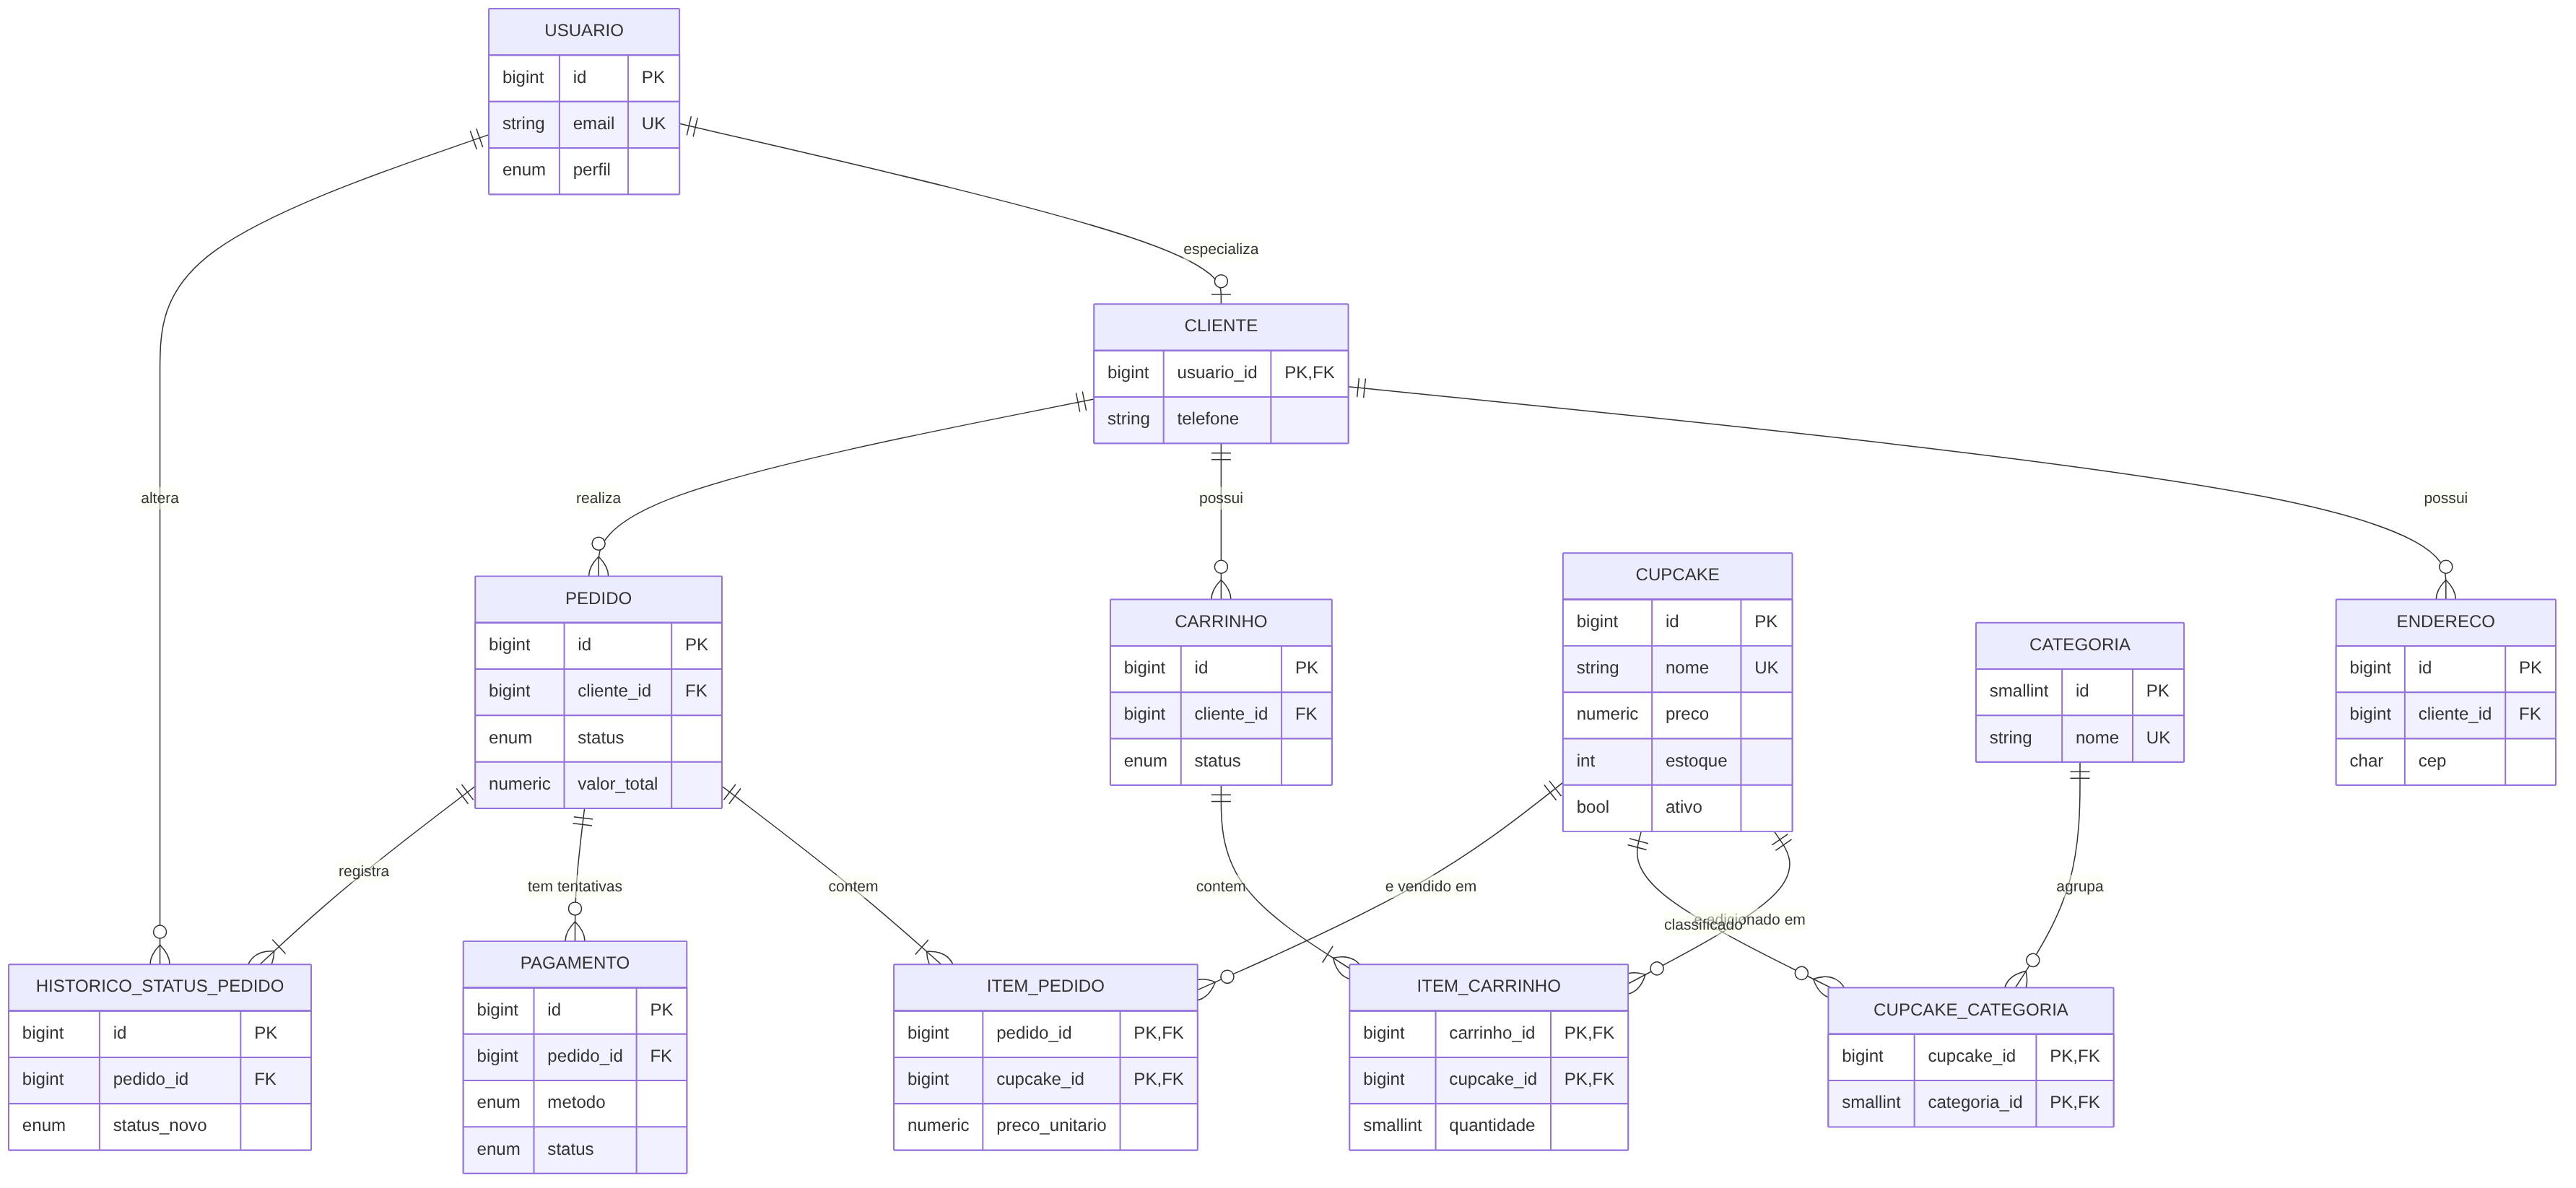
\includegraphics[width=\textwidth]{modelo_logico.png}
\caption{Modelo lógico relacional (entidades, chaves e cardinalidades)}
\end{figure}

\subsubsection{Esquemas relacionais}

Notação: \underline{sublinhado} indica chave primária e $\rightarrow$ indica chave estrangeira.

\begin{small}
\begin{itemize}
\item \textbf{usuario}(\underline{id}, nome, email, senha\_hash, perfil, ativo, criado\_em)
\item \textbf{cliente}(\underline{usuario\_id} $\rightarrow$ usuario, telefone)
\item \textbf{endereco}(\underline{id}, cliente\_id $\rightarrow$ cliente, apelido, cep, logradouro, numero, complemento, bairro, cidade, uf, principal, ativo)
\item \textbf{categoria}(\underline{id}, nome, ativa)
\item \textbf{cupcake}(\underline{id}, nome, descricao, ingredientes, preco, imagem\_url, estoque, destaque, ativo, criado\_em, atualizado\_em)
\item \textbf{cupcake\_categoria}(\underline{cupcake\_id} $\rightarrow$ cupcake, \underline{categoria\_id} $\rightarrow$ categoria)
\item \textbf{carrinho}(\underline{id}, cliente\_id $\rightarrow$ cliente, status, criado\_em, atualizado\_em)
\item \textbf{item\_carrinho}(\underline{carrinho\_id} $\rightarrow$ carrinho, \underline{cupcake\_id} $\rightarrow$ cupcake, quantidade)
\item \textbf{pedido}(\underline{id}, cliente\_id $\rightarrow$ cliente, status, data\_pedido, entrega\_cep, entrega\_logradouro, entrega\_numero, entrega\_complemento, entrega\_bairro, entrega\_cidade, entrega\_uf, taxa\_entrega, valor\_total, atualizado\_em)
\item \textbf{item\_pedido}(\underline{pedido\_id} $\rightarrow$ pedido, \underline{cupcake\_id} $\rightarrow$ cupcake, quantidade, preco\_unitario, subtotal)
\item \textbf{pagamento}(\underline{id}, pedido\_id $\rightarrow$ pedido, metodo, status, valor, gateway\_transacao\_id, criado\_em, processado\_em)
\item \textbf{transicao\_status\_pedido}(\underline{de}, \underline{para})
\item \textbf{historico\_status\_pedido}(\underline{id}, pedido\_id $\rightarrow$ pedido, status\_anterior, status\_novo, alterado\_por $\rightarrow$ usuario, alterado\_em)
\end{itemize}
\end{small}

\subsubsection{Normalização}

\begin{itemize}
\item \textbf{1FN:} todos os atributos são atômicos. O endereço foi decomposto em campos, e a lista \texttt{itens} da classe Carrinho virou uma tabela própria.
\item \textbf{2FN:} nas tabelas de chave composta (\texttt{item\_carrinho}, \texttt{item\_pedido}, \texttt{cupcake\_categoria}), os atributos dependem da chave inteira. O nome e o preço atual do produto ficam apenas em \texttt{cupcake}.
\item \textbf{3FN:} não há dependências transitivas. Categoria, cliente e produto são referenciados por chave, e não copiados.
\item \textbf{Desnormalizações intencionais:} \texttt{item\_pedido.preco\_unitario} e as colunas \texttt{entrega\_*} de \texttt{pedido} guardam o valor vigente na compra. Isso preserva o histórico mesmo que o preço ou o endereço mudem depois. \texttt{valor\_total} e \texttt{subtotal} são conferidos por regra de negócio.
\end{itemize}

\subsection{Modelo físico}

O script completo está no Apêndice A. Os principais elementos são:

\begin{itemize}
\item \textbf{Esquema} \texttt{loja}, com 13 tabelas.
\item \textbf{Tipos e domínios:} \texttt{status\_pedido}, \texttt{status\_pagamento}, \texttt{metodo\_pagamento}, \texttt{perfil\_usuario}, \texttt{status\_carrinho}, \texttt{d\_cep}, \texttt{d\_uf} e \texttt{d\_dinheiro}.
\item \textbf{Chaves primárias} do tipo \texttt{IDENTITY} e chaves compostas nas tabelas associativas.
\item \textbf{Índices únicos parciais:} um carrinho aberto por cliente, um endereço principal por cliente e um pagamento aprovado por pedido.
\item \textbf{Índices de desempenho} para a vitrine (RNF01), filtro por categoria (RNF02), pedidos por cliente e relatórios (RNF15).
\item \textbf{Triggers:} validação do fluxo de status (RN14), histórico automático, aprovação de pagamento que muda o pedido para PAGO, e atualização de \texttt{atualizado\_em}.
\item \textbf{Função} \texttt{fn\_confirmar\_pedido}: transforma o carrinho em pedido em uma única transação (copia preços e endereço, baixa o estoque e fecha o carrinho).
\item \textbf{Views:} \texttt{vw\_vitrine}, \texttt{vw\_carrinho\_detalhado}, \texttt{vw\_vendas\_diarias}, \texttt{vw\_produtos\_mais\_vendidos}, \texttt{vw\_estoque} e \texttt{vw\_pedidos\_resumo}.
\item \textbf{Segurança:} o papel \texttt{app\_loja} não pode apagar pedidos, itens, pagamentos nem histórico. Senhas são armazenadas somente como \textit{hash} (SHA-256 na versão do trabalho), e dados de cartão nunca são guardados (RNF08).
\end{itemize}

\subsubsection{Rastreabilidade das regras de negócio}

\begin{table}[H]
\centering
\small
\renewcommand{\arraystretch}{1.25}
\begin{tabular}{|c|p{5cm}|p{6.2cm}|}
\hline
\rowcolor{gray!40} \textbf{Regra} & \textbf{Descrição} & \textbf{Mecanismo no banco} \\ \hline
RN01 & Exibir apenas produtos ativos & Coluna \texttt{cupcake.ativo}, filtro em \texttt{vw\_vitrine} e índice parcial \\ \hline
RN02 & Categoria deve existir & FK de \texttt{cupcake\_categoria} para \texttt{categoria} \\ \hline
RN03 & Dados atualizados & Leitura direta da tabela; \texttt{atualizado\_em} via trigger \\ \hline
RN04 & Quantidade mínima 1 & \texttt{CHECK (quantidade >= 1)} em \texttt{item\_carrinho} \\ \hline
RN05 & Sem itens negativos & Mesmo \texttt{CHECK}; a remoção apaga a linha \\ \hline
RN06 & Valores consistentes & \texttt{vw\_carrinho\_detalhado} calcula subtotal e total no banco \\ \hline
RN07 & Endereço obrigatório & Colunas \texttt{NOT NULL}, domínios \texttt{d\_cep} e \texttt{d\_uf}; \texttt{fn\_confirmar\_pedido} exige endereço \\ \hline
RN08 & Métodos válidos & Tipo enumerado \texttt{metodo\_pagamento} (PIX, CARTAO) \\ \hline
RN09 & Pedido válido & \texttt{fn\_confirmar\_pedido} valida carrinho, estoque e produtos ativos \\ \hline
RN10 & Confirmar pagamento & Trigger que muda o pedido para PAGO quando o pagamento é APROVADO \\ \hline
RN11 & Status válido & Tipo enumerado \texttt{status\_pedido} \\ \hline
RN12 & Campos obrigatórios & \texttt{NOT NULL}, \texttt{CHECK (preco > 0)} e \texttt{UNIQUE (nome)} \\ \hline
RN13 & Produto existente & Edição por chave primária; produtos com pedidos não são apagados (\texttt{ON DELETE RESTRICT}) \\ \hline
RN14 & Fluxo correto & Tabela \texttt{transicao\_status\_pedido} e trigger de validação \\ \hline
RN15 & Dados atualizados & Views calculadas na consulta, sem tabela de cópia \\ \hline
\end{tabular}
\caption{Regras de negócio e como o banco as garante}
\end{table}

\subsection{Dicionário de dados}

Legenda: PK = chave primária; FK = chave estrangeira; UK = valor único. As colunas de data e hora usam \texttt{TIMESTAMPTZ}.

\subsubsection{Tabela \texttt{usuario}}
\noindent Generalização de Cliente e Administrador; guarda credenciais de acesso.\par\smallskip
\begingroup\footnotesize\renewcommand{\arraystretch}{1.2}
\begin{longtable}{|p{3.0cm}|p{2.6cm}|c|c|p{5.6cm}|}
\hline
\rowcolor{gray!40}\textbf{Coluna} & \textbf{Tipo} & \textbf{Chave} & \textbf{Nulo?} & \textbf{Descrição} \\ \hline
\endhead
\texttt{id} & BIGINT & PK & Não & Identificador do usuário \\ \hline
\texttt{nome} & VARCHAR(100) & -- & Não & Nome completo (mín. 2 caracteres) \\ \hline
\texttt{email} & VARCHAR(150) & UK & Não & E-mail de login (único, formato validado) \\ \hline
\texttt{senha\_hash} & VARCHAR(255) & -- & Não & Hash da senha (nunca texto puro) \\ \hline
\texttt{perfil} & perfil\_usuario & -- & Não & CLIENTE ou ADMINISTRADOR \\ \hline
\texttt{ativo} & BOOLEAN & -- & Não & Indica se a conta está ativa \\ \hline
\texttt{criado\_em} & TIMESTAMPTZ & -- & Não & Data/hora de criação \\ \hline
\end{longtable}
\endgroup
\subsubsection{Tabela \texttt{cliente}}
\noindent Especialização 1:1 de Usuario com dados exclusivos do cliente.\par\smallskip
\begingroup\footnotesize\renewcommand{\arraystretch}{1.2}
\begin{longtable}{|p{3.0cm}|p{2.6cm}|c|c|p{5.6cm}|}
\hline
\rowcolor{gray!40}\textbf{Coluna} & \textbf{Tipo} & \textbf{Chave} & \textbf{Nulo?} & \textbf{Descrição} \\ \hline
\endhead
\texttt{usuario\_id} & BIGINT & PK, FK & Não & Identificador do cliente (= usuario.id) (ref. usuario) \\ \hline
\texttt{telefone} & VARCHAR(15) & -- & Sim & Telefone apenas com dígitos (10 a 15) \\ \hline
\end{longtable}
\endgroup
\subsubsection{Tabela \texttt{endereco}}
\noindent Endereços de entrega salvos pelo cliente (US07).\par\smallskip
\begingroup\footnotesize\renewcommand{\arraystretch}{1.2}
\begin{longtable}{|p{3.0cm}|p{2.6cm}|c|c|p{5.6cm}|}
\hline
\rowcolor{gray!40}\textbf{Coluna} & \textbf{Tipo} & \textbf{Chave} & \textbf{Nulo?} & \textbf{Descrição} \\ \hline
\endhead
\texttt{id} & BIGINT & PK & Não & Identificador do endereço \\ \hline
\texttt{cliente\_id} & BIGINT & FK & Não & Cliente proprietário (ref. cliente) \\ \hline
\texttt{apelido} & VARCHAR(30) & -- & Sim & Nome amigável (ex.: Casa) \\ \hline
\texttt{cep} & d\_cep & -- & Não & CEP com 8 dígitos \\ \hline
\texttt{logradouro} & VARCHAR(150) & -- & Não & Rua/avenida \\ \hline
\texttt{numero} & VARCHAR(10) & -- & Não & Número do imóvel \\ \hline
\texttt{complemento} & VARCHAR(60) & -- & Sim & Complemento (opcional) \\ \hline
\texttt{bairro} & VARCHAR(80) & -- & Não & Bairro \\ \hline
\texttt{cidade} & VARCHAR(80) & -- & Não & Cidade \\ \hline
\texttt{uf} & d\_uf & -- & Não & Sigla do estado (2 letras maiúsculas) \\ \hline
\texttt{principal} & BOOLEAN & -- & Não & Endereço padrão (no máximo um ativo por cliente) \\ \hline
\texttt{ativo} & BOOLEAN & -- & Não & Exclusão lógica do endereço \\ \hline
\end{longtable}
\endgroup
\subsubsection{Tabela \texttt{categoria}}
\noindent Classificação dos cupcakes para filtro (US02).\par\smallskip
\begingroup\footnotesize\renewcommand{\arraystretch}{1.2}
\begin{longtable}{|p{3.0cm}|p{2.6cm}|c|c|p{5.6cm}|}
\hline
\rowcolor{gray!40}\textbf{Coluna} & \textbf{Tipo} & \textbf{Chave} & \textbf{Nulo?} & \textbf{Descrição} \\ \hline
\endhead
\texttt{id} & SMALLINT & PK & Não & Identificador da categoria \\ \hline
\texttt{nome} & VARCHAR(50) & UK & Não & Nome único (ex.: Vegano) \\ \hline
\texttt{ativa} & BOOLEAN & -- & Não & Categoria disponível para filtro \\ \hline
\end{longtable}
\endgroup
\subsubsection{Tabela \texttt{cupcake}}
\noindent Produto vendido na loja (US01, US03, US12, US13).\par\smallskip
\begingroup\footnotesize\renewcommand{\arraystretch}{1.2}
\begin{longtable}{|p{3.0cm}|p{2.6cm}|c|c|p{5.6cm}|}
\hline
\rowcolor{gray!40}\textbf{Coluna} & \textbf{Tipo} & \textbf{Chave} & \textbf{Nulo?} & \textbf{Descrição} \\ \hline
\endhead
\texttt{id} & BIGINT & PK & Não & Identificador do produto \\ \hline
\texttt{nome} & VARCHAR(100) & UK & Não & Nome único do cupcake \\ \hline
\texttt{descricao} & TEXT & -- & Não & Descrição exibida ao cliente \\ \hline
\texttt{ingredientes} & TEXT & -- & Sim & Lista de ingredientes \\ \hline
\texttt{preco} & NUMERIC(10,2) & -- & Não & Preço atual de venda ($>$ 0) \\ \hline
\texttt{imagem\_url} & VARCHAR(255) & -- & Sim & Endereço da imagem \\ \hline
\texttt{estoque} & INTEGER & -- & Não & Unidades disponíveis ($\geq$ 0) \\ \hline
\texttt{destaque} & BOOLEAN & -- & Não & Ordena a vitrine (CA03 da US01) \\ \hline
\texttt{ativo} & BOOLEAN & -- & Não & RN01: somente ativos aparecem na vitrine \\ \hline
\texttt{criado\_em} & TIMESTAMPTZ & -- & Não & Data/hora de cadastro \\ \hline
\texttt{atualizado\_em} & TIMESTAMPTZ & -- & Não & Última alteração (trigger) \\ \hline
\end{longtable}
\endgroup
\subsubsection{Tabela \texttt{cupcake\_categoria}}
\noindent Associação N:N entre cupcake e categoria.\par\smallskip
\begingroup\footnotesize\renewcommand{\arraystretch}{1.2}
\begin{longtable}{|p{3.0cm}|p{2.6cm}|c|c|p{5.6cm}|}
\hline
\rowcolor{gray!40}\textbf{Coluna} & \textbf{Tipo} & \textbf{Chave} & \textbf{Nulo?} & \textbf{Descrição} \\ \hline
\endhead
\texttt{cupcake\_id} & BIGINT & PK, FK & Não & Cupcake classificado (ref. cupcake) \\ \hline
\texttt{categoria\_id} & SMALLINT & PK, FK & Não & Categoria atribuída (ref. categoria) \\ \hline
\end{longtable}
\endgroup
\subsubsection{Tabela \texttt{carrinho}}
\noindent Carrinho persistido no banco (US04 a US06, RNF04).\par\smallskip
\begingroup\footnotesize\renewcommand{\arraystretch}{1.2}
\begin{longtable}{|p{3.0cm}|p{2.6cm}|c|c|p{5.6cm}|}
\hline
\rowcolor{gray!40}\textbf{Coluna} & \textbf{Tipo} & \textbf{Chave} & \textbf{Nulo?} & \textbf{Descrição} \\ \hline
\endhead
\texttt{id} & BIGINT & PK & Não & Identificador do carrinho \\ \hline
\texttt{cliente\_id} & BIGINT & FK & Não & Dono do carrinho (ref. cliente) \\ \hline
\texttt{status} & status\_carrinho & -- & Não & ABERTO, CONVERTIDO ou ABANDONADO (um ABERTO por cliente) \\ \hline
\texttt{criado\_em} & TIMESTAMPTZ & -- & Não & Criação \\ \hline
\texttt{atualizado\_em} & TIMESTAMPTZ & -- & Não & Última alteração (trigger) \\ \hline
\end{longtable}
\endgroup
\subsubsection{Tabela \texttt{item\_carrinho}}
\noindent Itens do carrinho (classe ItemCarrinho).\par\smallskip
\begingroup\footnotesize\renewcommand{\arraystretch}{1.2}
\begin{longtable}{|p{3.0cm}|p{2.6cm}|c|c|p{5.6cm}|}
\hline
\rowcolor{gray!40}\textbf{Coluna} & \textbf{Tipo} & \textbf{Chave} & \textbf{Nulo?} & \textbf{Descrição} \\ \hline
\endhead
\texttt{carrinho\_id} & BIGINT & PK, FK & Não & Carrinho (ref. carrinho) \\ \hline
\texttt{cupcake\_id} & BIGINT & PK, FK & Não & Produto (ref. cupcake) \\ \hline
\texttt{quantidade} & SMALLINT & -- & Não & RN04/RN05: mínimo 1 \\ \hline
\end{longtable}
\endgroup
\subsubsection{Tabela \texttt{pedido}}
\noindent Pedido confirmado (US09); guarda cópia do endereço de entrega.\par\smallskip
\begingroup\footnotesize\renewcommand{\arraystretch}{1.2}
\begin{longtable}{|p{3.0cm}|p{2.6cm}|c|c|p{5.6cm}|}
\hline
\rowcolor{gray!40}\textbf{Coluna} & \textbf{Tipo} & \textbf{Chave} & \textbf{Nulo?} & \textbf{Descrição} \\ \hline
\endhead
\texttt{id} & BIGINT & PK & Não & Número do pedido \\ \hline
\texttt{cliente\_id} & BIGINT & FK & Não & Cliente que comprou (ref. cliente) \\ \hline
\texttt{status} & status\_pedido & -- & Não & Situação atual (fluxo controlado por RN14) \\ \hline
\texttt{data\_pedido} & TIMESTAMPTZ & -- & Não & Data/hora da confirmação \\ \hline
\texttt{entrega\_cep} & d\_cep & -- & Não & CEP de entrega (cópia) \\ \hline
\texttt{entrega\_logradouro} & VARCHAR(150) & -- & Não & Rua de entrega (cópia) \\ \hline
\texttt{entrega\_numero} & VARCHAR(10) & -- & Não & Número de entrega (cópia) \\ \hline
\texttt{entrega\_complemento} & VARCHAR(60) & -- & Sim & Complemento (cópia) \\ \hline
\texttt{entrega\_bairro} & VARCHAR(80) & -- & Não & Bairro de entrega (cópia) \\ \hline
\texttt{entrega\_cidade} & VARCHAR(80) & -- & Não & Cidade de entrega (cópia) \\ \hline
\texttt{entrega\_uf} & d\_uf & -- & Não & UF de entrega (cópia) \\ \hline
\texttt{taxa\_entrega} & NUMERIC(10,2) & -- & Não & Taxa de entrega em R\$ \\ \hline
\texttt{valor\_total} & NUMERIC(10,2) & -- & Não & Itens + taxa de entrega em R\$ \\ \hline
\texttt{atualizado\_em} & TIMESTAMPTZ & -- & Não & Última alteração (trigger) \\ \hline
\end{longtable}
\endgroup
\subsubsection{Tabela \texttt{item\_pedido}}
\noindent Itens do pedido com preço congelado.\par\smallskip
\begingroup\footnotesize\renewcommand{\arraystretch}{1.2}
\begin{longtable}{|p{3.0cm}|p{2.6cm}|c|c|p{5.6cm}|}
\hline
\rowcolor{gray!40}\textbf{Coluna} & \textbf{Tipo} & \textbf{Chave} & \textbf{Nulo?} & \textbf{Descrição} \\ \hline
\endhead
\texttt{pedido\_id} & BIGINT & PK, FK & Não & Pedido (ref. pedido) \\ \hline
\texttt{cupcake\_id} & BIGINT & PK, FK & Não & Produto vendido (ref. cupcake) \\ \hline
\texttt{quantidade} & SMALLINT & -- & Não & Quantidade ($\geq$ 1) \\ \hline
\texttt{preco\_unitario} & NUMERIC(10,2) & -- & Não & Preço no momento da compra \\ \hline
\texttt{subtotal} & NUMERIC(10,2) & -- & Não & quantidade x preco\_unitario (coluna gerada) \\ \hline
\end{longtable}
\endgroup
\subsubsection{Tabela \texttt{pagamento}}
\noindent Tentativas de pagamento de um pedido (US08, US10).\par\smallskip
\begingroup\footnotesize\renewcommand{\arraystretch}{1.2}
\begin{longtable}{|p{3.0cm}|p{2.6cm}|c|c|p{5.6cm}|}
\hline
\rowcolor{gray!40}\textbf{Coluna} & \textbf{Tipo} & \textbf{Chave} & \textbf{Nulo?} & \textbf{Descrição} \\ \hline
\endhead
\texttt{id} & BIGINT & PK & Não & Identificador da tentativa \\ \hline
\texttt{pedido\_id} & BIGINT & FK & Não & Pedido pago (ref. pedido) \\ \hline
\texttt{metodo} & metodo\_pagamento & -- & Não & PIX ou CARTAO (RN08) \\ \hline
\texttt{status} & status\_pagamento & -- & Não & PENDENTE, APROVADO, RECUSADO ou ESTORNADO \\ \hline
\texttt{valor} & NUMERIC(10,2) & -- & Não & Valor cobrado ($>$ 0) \\ \hline
\texttt{gateway\_transacao\_id} & VARCHAR(100) & UK & Sim & ID da transação no gateway (único; sem dados de cartão) \\ \hline
\texttt{criado\_em} & TIMESTAMPTZ & -- & Não & Início da tentativa \\ \hline
\texttt{processado\_em} & TIMESTAMPTZ & -- & Sim & Retorno do gateway \\ \hline
\end{longtable}
\endgroup
\subsubsection{Tabela \texttt{transicao\_status\_pedido}}
\noindent Tabela de apoio com o fluxo válido de status (RN14).\par\smallskip
\begingroup\footnotesize\renewcommand{\arraystretch}{1.2}
\begin{longtable}{|p{3.0cm}|p{2.6cm}|c|c|p{5.6cm}|}
\hline
\rowcolor{gray!40}\textbf{Coluna} & \textbf{Tipo} & \textbf{Chave} & \textbf{Nulo?} & \textbf{Descrição} \\ \hline
\endhead
\texttt{de} & status\_pedido & PK & Não & Status de origem \\ \hline
\texttt{para} & status\_pedido & PK & Não & Status de destino permitido \\ \hline
\end{longtable}
\endgroup
\subsubsection{Tabela \texttt{historico\_status\_pedido}}
\noindent Auditoria das mudanças de status; alimenta o acompanhamento (US11).\par\smallskip
\begingroup\footnotesize\renewcommand{\arraystretch}{1.2}
\begin{longtable}{|p{3.0cm}|p{2.6cm}|c|c|p{5.6cm}|}
\hline
\rowcolor{gray!40}\textbf{Coluna} & \textbf{Tipo} & \textbf{Chave} & \textbf{Nulo?} & \textbf{Descrição} \\ \hline
\endhead
\texttt{id} & BIGINT & PK & Não & Identificador do registro \\ \hline
\texttt{pedido\_id} & BIGINT & FK & Não & Pedido (ref. pedido) \\ \hline
\texttt{status\_anterior} & status\_pedido & -- & Sim & Status antes da mudança (nulo na criação) \\ \hline
\texttt{status\_novo} & status\_pedido & -- & Não & Status após a mudança \\ \hline
\texttt{alterado\_por} & BIGINT & FK & Sim & Usuário responsável (ref. usuario) \\ \hline
\texttt{alterado\_em} & TIMESTAMPTZ & -- & Não & Data/hora da mudança \\ \hline
\end{longtable}
\endgroup


\subsubsection{Tipos enumerados}

\begin{table}[H]
\centering
\small
\renewcommand{\arraystretch}{1.25}
\begin{tabular}{|l|p{9cm}|}
\hline
\rowcolor{gray!40} \textbf{Tipo} & \textbf{Valores} \\ \hline
\texttt{perfil\_usuario} & CLIENTE, ADMINISTRADOR \\ \hline
\texttt{status\_carrinho} & ABERTO, CONVERTIDO, ABANDONADO \\ \hline
\texttt{status\_pedido} & AGUARDANDO\_PAGAMENTO, PAGO, EM\_PREPARO, ENVIADO, ENTREGUE, CANCELADO \\ \hline
\texttt{metodo\_pagamento} & PIX, CARTAO \\ \hline
\texttt{status\_pagamento} & PENDENTE, APROVADO, RECUSADO, ESTORNADO \\ \hline
\texttt{d\_cep} & CHAR(8), somente dígitos \\ \hline
\texttt{d\_uf} & CHAR(2), letras maiúsculas \\ \hline
\texttt{d\_dinheiro} & NUMERIC(10,2), valor $\geq$ 0 \\ \hline
\end{tabular}
\caption{Tipos enumerados e domínios}
\end{table}

\subsubsection{Fluxo permitido de status do pedido (RN14)}

\begin{center}
AGUARDANDO\_PAGAMENTO $\rightarrow$ PAGO $\rightarrow$ EM\_PREPARO $\rightarrow$ ENVIADO $\rightarrow$ ENTREGUE\\
\small Cancelamento (CANCELADO) é permitido a partir de AGUARDANDO\_PAGAMENTO, PAGO e EM\_PREPARO.
\end{center}

\subsection{Verificação do projeto físico}

O script foi executado em um PostgreSQL 16 sem erros, e os cenários abaixo foram testados, primeiro diretamente no banco e depois pela aplicação (API e telas), com os dados de carga inicial:

\begin{itemize}
\item vitrine com apenas produtos ativos e suas categorias, e filtro por categoria;
\item conversão do carrinho em pedido com baixa de estoque, preço congelado e total correto (itens mais taxa de entrega);
\item pagamento recusado seguido de nova tentativa aprovada, que muda o pedido para PAGO;
\item rejeição de transição inválida de status (de PAGO direto para ENTREGUE);
\item rejeição de quantidade zero, nome inválido, administrador cadastrado como cliente, e-mail ou nome de produto repetidos, e confirmação com carrinho vazio ou inexistente;
\item relatórios de vendas diárias, produtos mais vendidos e estoque;
\item bloqueio de \texttt{DELETE} em pedidos para o papel da aplicação;
\item acesso negado (403) de cliente às rotas do dono e (401) de visitante às rotas protegidas.
\end{itemize}

\newpage
\section{5ª Entrega: Implementação do Sistema}

Esta seção descreve como o sistema foi construído a partir dos artefatos das entregas anteriores. O passo a passo de instalação e uso está no documento separado \textit{Manual de Uso}. Os diagramas UML revisados e o modelo conceitual estão no documento \textit{Revisão da Modelagem UML e Projeto Conceitual de Dados}, e os testes automatizados (131 casos de back-end e banco e 31 de interface, todos aprovados) estão descritos no \textit{Documento de Testes}.

\subsection{Repositório}

O código-fonte da implementação (padrão MVC em Java), o banco de dados, os testes automatizados e a documentação estão no GitHub:

\begin{center}\url{https://github.com/Fellp-coffww/Loja-Cupcake}\end{center}

\begin{table}[H]
\centering\small\renewcommand{\arraystretch}{1.3}
\begin{tabular}{|p{4.2cm}|p{9.4cm}|}
\hline
\rowcolor{gray!40} \textbf{Pasta ou arquivo} & \textbf{Conteúdo} \\ \hline
\texttt{src/loja/} & Back-end: \texttt{model}, \texttt{dao}, \texttt{controller} e \texttt{util} (MVC) e \texttt{Main.java} \\ \hline
\texttt{public/} & Front-end (View): páginas, scripts e estilos \\ \hline
\texttt{sql/} & Esquema, regras, \textit{triggers}, \textit{views} e dados iniciais do PostgreSQL \\ \hline
\texttt{test/} e \texttt{testes/} & Testes automatizados de back-end (JUnit) e de interface (Playwright) \\ \hline
\texttt{docs/} & Manual de uso, documento do banco de dados, revisão UML e modelo conceitual, documento de testes \\ \hline
\texttt{README.md} & Como instalar, executar e testar \\ \hline
\end{tabular}
\caption{Organização do repositório}
\end{table}

\subsection{Tecnologias}

\begin{itemize}
\item \textbf{Back-end:} Java 17 ou superior, sem frameworks. O servidor HTTP é o que já acompanha o JDK (\texttt{com.sun.net.httpserver}) e o acesso ao banco usa JDBC com o driver oficial do PostgreSQL 42.7.
\item \textbf{Banco de dados:} PostgreSQL 16, conforme o projeto da seção anterior.
\item \textbf{Front-end:} HTML, CSS e JavaScript puros, sem bibliotecas, servidos pelo próprio back-end.
\item \textbf{Formato de troca de dados:} JSON, com conversor próprio mínimo.
\end{itemize}

\subsection{Arquitetura MVC}

\begin{table}[H]
\centering
\small
\renewcommand{\arraystretch}{1.3}
\begin{tabular}{|p{2.2cm}|p{4.3cm}|p{7.2cm}|}
\hline
\rowcolor{gray!40} \textbf{Camada} & \textbf{Local} & \textbf{Responsabilidade} \\ \hline
Model & \texttt{model/} e \texttt{dao/} & Registros (Cupcake, Pedido, Endereco etc.) e acesso ao banco por DAOs com \textit{PreparedStatement} \\ \hline
View & \texttt{public/} & Telas \texttt{index.html} (cliente) e \texttt{admin.html} (dono), com JavaScript e CSS \\ \hline
Controller & \texttt{controller/} & Recebem as requisições de \texttt{/api/...}, validam os dados, chamam os DAOs e devolvem JSON \\ \hline
Apoio & \texttt{util/} e \texttt{Main.java} & Conexão, JSON, sessão, hash de senha, respostas HTTP e registro das rotas \\ \hline
\end{tabular}
\caption{Organização do código em MVC}
\end{table}

Fluxo de uma requisição: o navegador (View) chama \texttt{fetch('/api/...')}, o Controller valida e delega ao DAO, o DAO consulta o PostgreSQL e o resultado volta em JSON para a View.

As regras de negócio mais sensíveis ficam no banco (quantidade mínima, fluxo de status do pedido, baixa de estoque, histórico). O Controller só valida o formato dos dados e traduz os erros do banco em mensagens claras em português.

\subsection{Telas e navegação}

O mapa navegacional da 3ª entrega foi adaptado na implementação:

\begin{enumerate}
\item \textbf{Login:} ao abrir o endereço, é a única tela exibida, com as abas ``Entrar'' e ``Criar conta''.
\item \textbf{Loja:} após o login, aparece a vitrine com filtro por categoria e janela de detalhes do produto.
\item \textbf{Aba lateral:} painel deslizante à direita, com duas abas: ``Carrinho'' (itens, total e botão \textit{Finalizar pedido}) e ``Meus pedidos'' (status e pagamento).
\item \textbf{Finalizar pedido:} janela para escolher ou cadastrar o endereço e confirmar.
\item \textbf{Pagamento:} janela com PIX ou cartão, aberta após a confirmação ou pelo botão \textit{Pagar agora}.
\item \textbf{Painel do dono} (\texttt{admin.html}): dashboard, pedidos com troca de status, cadastro e edição de produtos. O administrador é levado a esse painel ao fazer login.
\end{enumerate}

\subsection{Interface de programação (API REST)}

\small
\begin{longtable}{|p{7.9cm}|p{1.7cm}|p{3.0cm}|}
\hline
\rowcolor{gray!40} \textbf{Método e rota} & \textbf{Acesso} & \textbf{Histórias} \\ \hline
\endhead
\texttt{GET /api/cupcakes[?categoria=ID]} & Público & US01, US02 \\ \hline
\texttt{GET /api/cupcakes/\{id\}} & Público & US03 \\ \hline
\texttt{GET /api/categorias} & Público & US02 \\ \hline
\texttt{POST /api/cadastro, /api/login, /api/logout} & Público & Acesso \\ \hline
\texttt{GET /api/carrinho} & Cliente & US06 \\ \hline
\texttt{POST /api/carrinho/itens} & Cliente & US04 \\ \hline
\texttt{DELETE /api/carrinho/itens/\{id\}} & Cliente & US05 \\ \hline
\texttt{GET, POST /api/enderecos} & Cliente & US07 \\ \hline
\texttt{POST /api/pedidos} & Cliente & US09 \\ \hline
\texttt{POST /api/pedidos/\{id\}/pagamento} & Cliente & US08, US10 \\ \hline
\texttt{GET /api/pedidos} & Cliente & US11 \\ \hline
\texttt{GET, POST /api/admin/cupcakes} & Dono & US12 \\ \hline
\texttt{PUT /api/admin/cupcakes/\{id\}} & Dono & US13 \\ \hline
\texttt{GET /api/admin/pedidos} & Dono & US14 \\ \hline
\texttt{PUT /api/admin/pedidos/\{id\}/status} & Dono & US14 \\ \hline
\texttt{GET /api/admin/dashboard} & Dono & US15 \\ \hline
\end{longtable}

\subsection{Autenticação e segurança}

\begin{itemize}
\item O login devolve um \textit{token} que o navegador envia no cabeçalho \texttt{Authorization}. As sessões ficam em memória no servidor.
\item Cada rota exige o perfil correto: rotas do cliente só aceitam CLIENTE e rotas \texttt{/api/admin} só aceitam ADMINISTRADOR (resposta 403 nos demais casos).
\item As senhas são guardadas apenas como \textit{hash} SHA-256; em produção recomenda-se bcrypt ou argon2.
\item Todas as consultas usam parâmetros (\textit{PreparedStatement}), o que evita injeção de SQL. O front-end escapa o texto exibido para evitar injeção de HTML.
\item Dados de cartão não são solicitados nem armazenados.
\end{itemize}

\subsection{Rastreabilidade: histórias de usuário e implementação}

\begin{longtable}{|p{4.2cm}|c|p{7.4cm}|}
\hline
\rowcolor{gray!40} \textbf{História} & \textbf{Situação} & \textbf{Observação} \\ \hline
\endhead
US01 Vitrine & Completa & Somente produtos ativos, ordenados por destaque \\ \hline
US02 Filtro por categoria & Completa & Atualização imediata da lista \\ \hline
US03 Detalhes & Completa & Descrição, ingredientes, imagem e preço \\ \hline
US04 Adicionar ao carrinho & Parcial & Cada clique soma uma unidade; a API aceita quantidade, mas a tela ainda não tem seletor \\ \hline
US05 Remover item & Parcial & Remove o item sem pedir confirmação (prevista no CU05) \\ \hline
US06 Visualizar carrinho & Completa & Subtotal por item e total \\ \hline
US07 Endereço de entrega & Parcial & Validação e gravação funcionam; falta a consulta automática ao ViaCEP (T7.2) \\ \hline
US08 Forma de pagamento & Completa & PIX ou cartão \\ \hline
US09 Confirmar pedido & Parcial & Pedido criado em transação única; falta tela de revisão final (T9.1) \\ \hline
US10 Processar pagamento & Parcial & Gateway simulado, com opção de recusa para demonstração; sem \textit{webhook} (T10.2) \\ \hline
US11 Acompanhar pedido & Parcial & Atualização periódica (15 s), sem tempo real \\ \hline
US12 Cadastrar produto & Completa & Imagem informada por URL \\ \hline
US13 Editar produto & Completa & Inclui ativar, desativar e ajustar estoque \\ \hline
US14 Atualizar status & Completa & Fluxo validado pelo banco (RN14) \\ \hline
US15 Dashboard de vendas & Parcial & Tabelas de vendas, mais vendidos e estoque; sem gráficos (T15.1) \\ \hline
\end{longtable}

\subsection{Testes automatizados}

O sistema tem testes automatizados em cinco níveis: unitário (conversor JSON, senha e sessão), integração dos DAOs com o PostgreSQL, regras do próprio banco, API de ponta a ponta e interface no navegador. Todos são repetíveis com os scripts \texttt{testar.bat} e \texttt{testar\_interface.py}. Os testes encontraram dois defeitos de tratamento de entrada (JSON cortado e número decimal em campo inteiro), já corrigidos.

\subsection{Simplificações e trabalhos futuros}

\begin{itemize}
\item Integrar um gateway de pagamento real em modo de testes (\textit{sandbox}) e tratar o \textit{webhook}.
\item Consultar o CEP no ViaCEP e preencher o endereço automaticamente.
\item Seletor de quantidade no carrinho, tela de revisão antes de confirmar o pedido e gráficos no dashboard.
\item Entrada de estoque com histórico de movimentações e devolução ao estoque em pedidos cancelados.
\end{itemize}


\newpage
\appendix
\section{Script SQL completo (PostgreSQL)}

\begingroup
\fvset{fontsize=\tiny, breaklines=true, numbers=left, numbersep=4pt}
\VerbatimInput{schema_loja_cupcakes.sql}
\endgroup

\end{document}